\chapter{Conceptes previs}\label{ch:conceptes_previs}

En aquest capítol es descriuen els conceptes bàsics necessaris per tal d'entendre com s'han dut a terme les diferents etapes del projecte i sense els quals no seria possible entendre els continguts dels capítols posteriors.

\section{Espectrofotometria per a la detecció d'agents contaminants}\label{sec:espectrofotometria_per_a_la_detecció_d'agents_contaminants}

L'espectrofotometria és una tècnica analítica utilitzada per determinar concentracions de determinats compostos en solució. El principi físic que permet l'ús d'aquesta tècnica és la transmitància explicada per la llei de \textit{Lambert-Beer} i es basa en el fet que les molècules absorbeixen radiació electromagnètica. Aquest tipus d'anàlisi s'acostuma a realitzar amb un espectrofotòmetre que permet seleccionar longituds d'ona específiques per fer-les passar a través d'una mostra i mesurar-ne la quantitat de llum absorbida.

Aquest projecte es basa íntegrament en l'ús de l'espectrofotometria per a detectar agents contaminants en mostres d'aigua. Utilitza la llei de \textit{Lambert-Beer} per a analitzar el senyal lumínic que passa pel medi aquós.

\subsection{Transmitància i llei de \textit{Lambert-Beer}}\label{subsec:lambert-beer}

La transmitància és la relació entre la intensitat de llum d'entrada i sortida en un medi per a una longitud d'ona específica. Matemàticament s'expressa en forma de fracció i està governada per la llei de \textit{Lambert-Beer} (eq. \ref{eq:lambert-beer}) que permet obtenir informació sobre la concentració de certes molècules en solució.

\begin{equation}\label{eq:lambert-beer}
\frac{\acs{II}}{\acs{IO}} = e^{-\acs{ALPHA}\acs{c}\acs{L}}
\end{equation}

$ \acsu{II} $ és la intensitat espectral d'entrada mentre que $ \acsu{IO} $ la intensitat espectral de sortida. $ \acsu{ALPHA} $ és el coeficient d'absorció molar, $ \acsu{c} $ la concentració molar i $ \acsu{L} $ la longitud del camí òptic. Els paràmetres \ac{ALPHA} i \ac{L} es poden fixar per a cada experiment deixant \ac{c} com a única variable. Aquesta equació es pot expressar també en termes d'absorbància (\acsu{A}):

\begin{equation}
\acs{A} = -\ln\left(\frac{\acs{II}}{\acs{IO}}\right) = \acs{ALPHA}\acs{c}\acs{L}
\end{equation}

\subsection{Bioassajos microbiològics de toxicitat}\label{subsec:bioassajos_microbiològics_de_toxicitat}

Un protocol comú per a determinar de forma no selectiva la presència d'agents contaminants potencialment tòxics en una mostra es basa en l'incubació d'organismes vius, com ara bacteris o algues, i avaluar-ne la viabilitat \cite{oanh:1995,tizzard:2004}. 

Una de les estratègies més acceptada consisteix en estudiar el metabolisme ce\lgem ular mitjançant un reactiu extern. Per aquest tipus d'estudis, és força comú utilitzar ferricianur, un compost de color groc intens, que interacciona amb citocroms i altres proteïnes de membrana involucrades en la respiració ce\lgem ular per reduir-se a ferrocianur (eq. \ref{eq:fecn}), una molècula incolora \cite{morris:2001,liu:2009,catterall:2010,li:2013,yip:2014}.

\begin{equation}\label{eq:fecn}
	\ce{\underset{\textit{ferricianur}}{\ce{[Fe(CN)_{6}]^{-3}}} ->[\textit{no-tòxics}][\textit{respiració ce\lgem ular}] \underset{\textit{ferrocianur}}{\ce{[Fe(CN)_{6}]^{-4}}}}
\end{equation}

En una mostra sense tòxics no hi haurà cap impediment per a què el metabolisme bacterià dugui a terme aquesta reacció i la mostra perdrà progressivament el color groc. En presència d'un tòxic, però, el procés de respiració és alterat i aquesta reducció no es produeix tant eficaçment, mantenint en cert grau el color groc.

Es pot analitzar la cinètica d'aquesta reacció per fer un estudi quantitatiu de toxicitat general. Aquest bioassaig òptic s'ha desenvolupat al laboratori de Microbiologia Ambiental de la \ac{UAB} i serà el mètode per a la detecció quantitativa i simple de productes tòxics en aigua utilitzat pel sistema explicat en el present treball.

\section{Característiques del projecte}

Es requereix un dispositiu capaç de realitzar un bioassaig de toxicitat general com el descrit en l'\hyperref[subsec:bioassajos_microbiològics_de_toxicitat]{apartat anterior} utilitzant el concepte de \ac{LOC}. Això vol dir es necessita un dispositiu simple, petit i fàcil de manejar, molt diferent als espectrofotòmetres de laboratori. 

El punt crític és aconseguir aïllar el raig de llum que travessa la mostra per evitar interferències. Els espectrofotòmetres convencionals ho fan utilitzant un espai tancat amb un làser que emet a una freqüència determinada. La solució proposada és utilitzar un díode emissor de llum (\acsu{LED}) que emeti un senyal sinusoïdal fàcilment filtrable electrònicament i traduir-lo a un nivell de tensió representatiu de la transmitància.

\section{Dispositius i circuits electrònics}\label{sec:components_circuits_electronics}

En el present treball apareixen una sèrie de components electrònics que permeten tant la generació d'un senyal lumínic com el tractament d'aquest un cop ha interaccionat amb el medi aquós.

\subsection{Díode}\label{subsec:diode}

Un díode és un dispositiu electrònic no lineal i polaritzat que només permet la circulació del corrent en un sentit. És important destacar les  propietats òptiques que presenten els \ac{LED} i els fotodíodes ja que tenen un paper de pes en aquest sistema de detecció d'agents contaminants.

\begin{itemize}
	
	\item{\textbf{\ac{LED}: }}No deixa de comportar-se electrònicament com un díode però té la característica que emet llum incoherent d'espectre reduït quan hi circula corrent en directa. El color depèn del material del qual està format.
	
	\item{\textbf{Fotodíode: }}Generalment estan connectats en inversa i generen una petita quantitat de corrent quan són excitats amb llum incident. Es poden comportar com a cè\lgem ules fotovoltaiques.
	
\end{itemize}

Una característica molt important que comparteixen tots els díodes és la tensió llindar (\acsu{VT}) que impedeix la circulació del corrent mentre la tensió entre els dos elèctrodes no arriba a un cert valor, generalment al voltant de \SI{0.7}{\volt} però se'n poden trobar de tot tipus. Aquesta característica fa referència al comportament dels díodes quan estan connectats en directa però també disposen d'una tensió de ruptura (\acsu{VB}) quan estan connectats en inversa per sobre de la qual es provocarà un efecte allau i circularan grans quantitats de corrent en sentit oposat.

\subsection{Divisor de tensió}\label{subsec:divisor_tensio}

Un divisor de tensió és un circuit que permet reduir el voltatge d'entrada (\acsu{VIN}) a una fracció d'aquest mitjançant una sèrie de resistors (fig. \ref{fig:schematic_divisor_tensio}). Pel correcte funcionament s'ha de poder negligir el corrent de sortida. En aquest sistema no serà un problema ja que totes les tensions obtingudes mitjançant un divisor de tensió van directes a una de les entrades d'un \ac{OPAMP}.

\begin{figure}[htp]
	\centering
	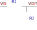
\includegraphics[width=0.25\textwidth]{Figures/schematic_divisor_tensio.pdf}
	\caption[Divisor de tensió]{Schematic\textit{ d'un divisor de tensió}\\{\footnotesize La tensió de sortida (\acsu{VOUT}) es pot obtenir mitjançant l'equació \ref{eq:divisor}.}}
	\label{fig:schematic_divisor_tensio}
\end{figure}

\begin{equation}\label{eq:divisor}
	\acs{VOUT} = \frac{\acs{R}_{2}}{\acs{R}_{1} + \acs{R}_{2}}\acs{VIN}
\end{equation}

\subsection{Circuit rectificador}\label{subsec:circuit_rectificador}

El tipus de rectificador que interessa per aquest sistema és un detector d'envolupant que utilitzi un díode per deixar passar només el punts del senyal superiors a \ac{VT} i, mitjançant un circuit \acsu{RC}, es pot aconseguir que la tensió de sortida sigui equivalent al valor màxim del senyal altern (fig. \ref{fig:grafica_senyal}).

Un circuit \ac{RC} està compost per resistors i condensadors i serveix principalment per filtrar senyals. S'encarrega de frenar el decaïment de la tensió quan la senyal d'entrada es redueix degut al comportament sinusoïdal. Si s'ajusta correctament, pot ajudar el circuit rectificador a tenir un nivell de tensió relativament estable en la sortida enlloc de la mitja ona sinusoïdal que permet passar el díode.

\begin{figure}[htp]
	\centering
	\includegraphics[width=0.8\textwidth]{Figures/wave_graph.pdf}
	\caption[Gràfica de l'efecte del detector d'envolupant]{Schematic\textit{ d'un divisor de tensió}\\{\footnotesize La tensió de sortida (\acsu{VOUT}) es pot obtenir mitjançant l'equació \ref{eq:divisor}.}}
	\label{fig:grafica_senyal}
\end{figure}

\subsection{\acl{OPAMP}}\label{subsec:amplificador_operacioanl}

Un \ac{OPAMP} és un circuit integrat amb dos entrades (una inversora i una altra no-inversora) i una sortida determinada per la diferència entre les dos entrades multiplicada per un guany. Una de les funcions principals que se'ls va detectar en un principi i de la qual els prové el nom és la de computar operacions matemàtiques bàsiques analògicament. 

%\footnote{Ens els \acp{OPAMP}, el guany en llaç obert (sense realimentació negativa) es pot considerar indefinidament gran. Aquest fet fa que, si no es realimenten, estiguin pràcticament sempre saturats.}

Són uns dispositius actius formats per transistors, resistors i condensadors que necessiten estar contínuament alimentats per una font de tensió per funcionar. Tenen un rang dinàmic sempre dintre de la diferència de tensió que produeix la font. Els \acp{OPAMP} \textit{rail-to-rail} utilitzats en aquest projecte tenen la característica especial que permeten justament arribar a aquests límits (o carrils) de tensió establerts per les fonts a diferència dels convencionals que acostumen a quedar-se a un cert voltatge.

Els amplificadors tenen una sèrie de característiques que condicionen el seu comportament:

\begin{itemize}
	
	\item{\textbf{Guany de llaç obert infinit: }}Explica el comportament com a comparador. En funció de quina de les tensions d'entrada sigui més gran, la sortida es saturarà pel límit superior o inferior del rang dinàmic.
	
	\item{\textbf{Impedància d'entrada infinita: }}Pels terminals \acsu{V+} i \acsu{V-} no hi circula corrent.
	
	\item{\textbf{Impedància de sortida nula: }}Es pot obtenir qualsevol nivell de tensió dintre del rang dinàmic independentment de la càrrega que circuli.
	
\end{itemize}

A partir d'aquestes característiques, si es connecta la sortida de l'\ac{OPAMP} amb l'entrada inversora, es forma una configuració especial anomenada realimentació negativa. En aquesta disposició, es força que les tensions d'entrada siguin iguals ($ \acsu{V+} = \acsu{V-} $) i la tensió de sortida (\ac{VOUT}) no estarà sempre saturada. En funció de quins components electrònics es posin i en quina disposició, l'amplificador tindrà una sèrie d'aplicacions molt interessants.

\begin{itemize}
	\item{\textbf{Amplificador de transimpedància (\ac{TIA}): }}Serveix per transformar un senyal de corrent en un senyal de tensió mitjançant l'equació \ref{eq:tia}. Cal destacar el signe negatiu ja que si es vol una \ac{VOUT} positiva caldrà que la intensitat d'entrada (\acsu{IIN}) sigui en sentit negatiu (fig. \ref{fig:schematic_transimpedancia}).
	
	\begin{equation}\label{eq:tia}
	\acs{VOUT} = -\acs{IIN}\acs{R}
	\end{equation}
	
	\begin{figure}[htp]
		\centering
		\includegraphics[width=0.4\textwidth]{Figures/schematic_transimpedancia.pdf}
		\caption[Amplificador de transimpedància]{Schematic\textit{ d'un amplificador de transimpedància}}
		\label{fig:schematic_transimpedancia}
	\end{figure}
	
	\item {\textbf{Circuit integrador: }}Serveix per realitzar l'operació matemàtica d'integració mitjançant l'equació \ref{eq:integrador}.
	
	\begin{equation}\label{eq:integrador}
	\acs{VOUT} = -\frac{\num{1}}{\acs{R}\acs{C}}\int_{\num{0}}^{\acs{T}}\acs{VIN}
	\end{equation}
	
	\begin{figure}[htp]
		\centering
		\includegraphics[width=0.4\textwidth]{Figures/schematic_integrator.pdf}
		\caption[Amplificador integrador]{Schematic\textit{ d'un amplificador integrador}}
		\label{fig:schematic_integrador}
	\end{figure}
	
	\item{\textbf{Circuit multiplicador: }}La multiplicació de dos tensions d'entrada és operació matemàtica més difícil de realitzar analògicament, es poden utilitzar quatre \acp{OPAMP} en la disposició de la figura \ref{fig:schematic_multiplicador_4}. Els dos primers són amplificadors logarítmics, el del mig és sumador inversor i l'últim és exponencial, això ens permet fer ús de les propietats dels logaritmes per realitzar la multiplicació. L'operacional complet es pot resoldre amb la següent equació si es fan un cert nombre d'assumpcions en el disseny:
	
	\begin{figure}[htp]
		\centering
		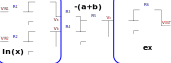
\includegraphics[width=0.8\textwidth]{Figures/schematic_multiplicador_4.pdf}
		\caption[Circuit multiplicador complet]{Schematic\textit{ d'un circuit multiplicador complet}\\{\footnotesize La tensió de sortida (\acs{VOUT}) es pot obtenir mitjançant l'equació \ref{eq:multiplicador} si es considera $ \acs{R}_{1} = \acs{R}_{2} $, $ \acs{R}_{3} = \acs{R}_{4} = \acs{R}_{5} $ i que tots els díodes són iguals.}}
		\label{fig:schematic_multiplicador_4}
	\end{figure}

	\begin{equation}
	\acs{V}_{a} = -\acs{N}\acs{Vt}\ln\left(\dfrac{\acs{VIN}_{\num{1}}}{\acs{R}_{1}\acs{IS}}\right) \qquad \acs{V}_{b} = -\acs{N}\acs{Vt}\ln\left(\dfrac{\acs{VIN}_{\num{2}}}{\acs{R}_{2}\acs{IS}}\right)
	\end{equation}
	
	\begin{equation}
	\acs{V}_{c} = -\acs{R}_{\num{5}}\left(\frac{\acs{V}_{a}}{\acs{R}_{\num{3}}}+\frac{\acs{V}_{b}}{\acs{R}_{\num{4}}}\right) 
	\end{equation}
	
	\begin{equation}\label{eq:multiplicador}
	\acs{VOUT} = -\acs{R}_{\num{6}}\acs{IS}e^{\frac{\acs{V}_{c}}{\acs{N}\acs{Vt}}} = -\frac{\acs{R}_{6}}{\acs{R}_{1}}\acs{VIN}_{1}\acs{VIN}_{2}
	\end{equation}
	
	\item{\textbf{Filtre \textit{biquad Sallen-Key}: }}Són un tipus de filtres actius\footnote{Estan fets amb un \ac{OPAMP} i, per tant, necessiten alimentació externa.} de segon ordre\footnote{Un filtre de primer ordre té una resposta freqüencial que redueix \SI{20}{\decibel/dècada} mentre que un de segon ordre redueix \SI{40}{\decibel/dècada}, sent més efectiu per al filtratge de senyals no desitjats.}. L'arquitectura \textit{Sallen-Key} inclou una realimentació positiva (a més de la negativa) a un circuit \ac{RC} anomenada \textit{biquad} (fig. \ref{fig:schematic_sallen-key}). Si es volgués augmentar l'ordre d'aquest tipus de filtre només caldria connectar un altre filtre en cascada \cite{kendall:2007}.
	
	\begin{figure}[htp]
		\centering
		\includegraphics[width=0.5\textwidth]{Figures/schematic_sallen-key.pdf}
		\caption[Esquema general d'un filtre amb configuració \textit{biquad}]{\textit{Esquema general d'un filtre amb configuració }biquad\\{\footnotesize Els components \acsu{Z} poden ser resistors o condensadors i el filtre serà passa-baix, passa-alt o passa-banda en funció de la distribució d'aquests.}}
		\label{fig:schematic_sallen-key}
	\end{figure}

	El factor de qualitat (\acsu{Q}) es pot calcular amb l'equació \ref{eq:qf} i determinarà factors importants com ara la freqüència de ressonància del circuit o l'amplada de banda.
	
	\begin{eqfloat}%[htp]
		\begin{equation}
		\acs{Q} = \frac{\acs{F0}}{\acs{F}_{màx} - \acs{F}_{min}} = \frac{\acs{F0}}{\acs{AB}}
		\end{equation}
		\caption{\acsu{F0} és la freqüència central i \acsu{AB} és l'amplada de banda.}
		\label{eq:qf}
	\end{eqfloat}
	
	\item{\textbf{Super-díode: }}Es pot obtenir un díode que es comporti idealment mitjançant un \ac{OPAMP}. Això equival a tenir $ \ac{VT} = \SI{0}{\volt} $ però, com que és un dispositiu actiu, necessita ser alimentat. La configuració bàsica es pot veure en la figura \ref{fig:schematic_superdiode}.
	
	\begin{figure}[htp]
		\centering
		\includegraphics[width=0.4\textwidth]{Figures/schematic_superdiode.pdf}
		\caption[Super-díode]{Schematic\textit{ d'un super-díode}}
		\label{fig:schematic_superdiode}
	\end{figure}
		
\end{itemize}

\section{Plataforma \textit{Arduino}}\label{sec:plataforma_arduino}

\textit{Arduino} és una plataforma de maquinari lliure que ofereix plaques amb un microcontrolador fàcil de programar i amb moltes possibilitats d'adaptar-se a tota mena de petits projectes d'electrònica i robòtica.  Hi ha molts models de plaques però totes incorporen una sèrie de pins que permeten el fàcil control de circuits. Un concepte molt estès és l'ús de mòduls d'expansió o \textit{shields} que es munten directament sobre la placa principal i incorporen funcionalitats que amplien les capacitats de l'\textit{Arduino}.

\subsection{\textit{Arduino DUE}}\label{subsec:arduino}

Aquest model de placa és més gran que el model més comercialitzat degut a que incorpora una sèrie de funcionalitats extra a part de incorporar un microprocessador més potent. Entre elles s'hi inclouen algunes necessàries per al desenvolupament d'aquest projecte com ara el \acs{DAC}.

\begin{figure}[htp]
\centering
\includegraphics[width=0.8\textwidth]{Figures/arduino_due.png}
\caption[Arduino DUE]{\textit{Arduino DUE}}
\label{fig:arduino_due}
\end{figure}
